
\chapter{Experimental Method}
\label{chap:experimental_method}


\section{Development of Linear Motion Platform}
\label{sec:development_of_linear_motion_platform}

A robotic linear motion platform was developed using Lego\textsuperscript{\textregistered} Mindstorms\textsuperscript{\textregistered} parts.
The platform was designed to carry a Lytro camera and a Nikon D5100 DSLR camera side-by-side.
Support for both cameras was made out of Lego parts.
The motion platform consisted of a wheeled based that carried the cameras.
It was attached by thread to a drum, driven by two Mindstorms motors.
The drum was manually held in place during operation, and the Matlab RWHT NXT Toolbox \cite{rwth2007toolbox} was used to interface with the motors.

The angular velocity of the drum was empirically calibrated allowing a desired velocity and linear distance to set in software.
Figure \ref{fig:motion_platform} shows the design of the linear motion platform.

\begin{figure}[h]
\centering
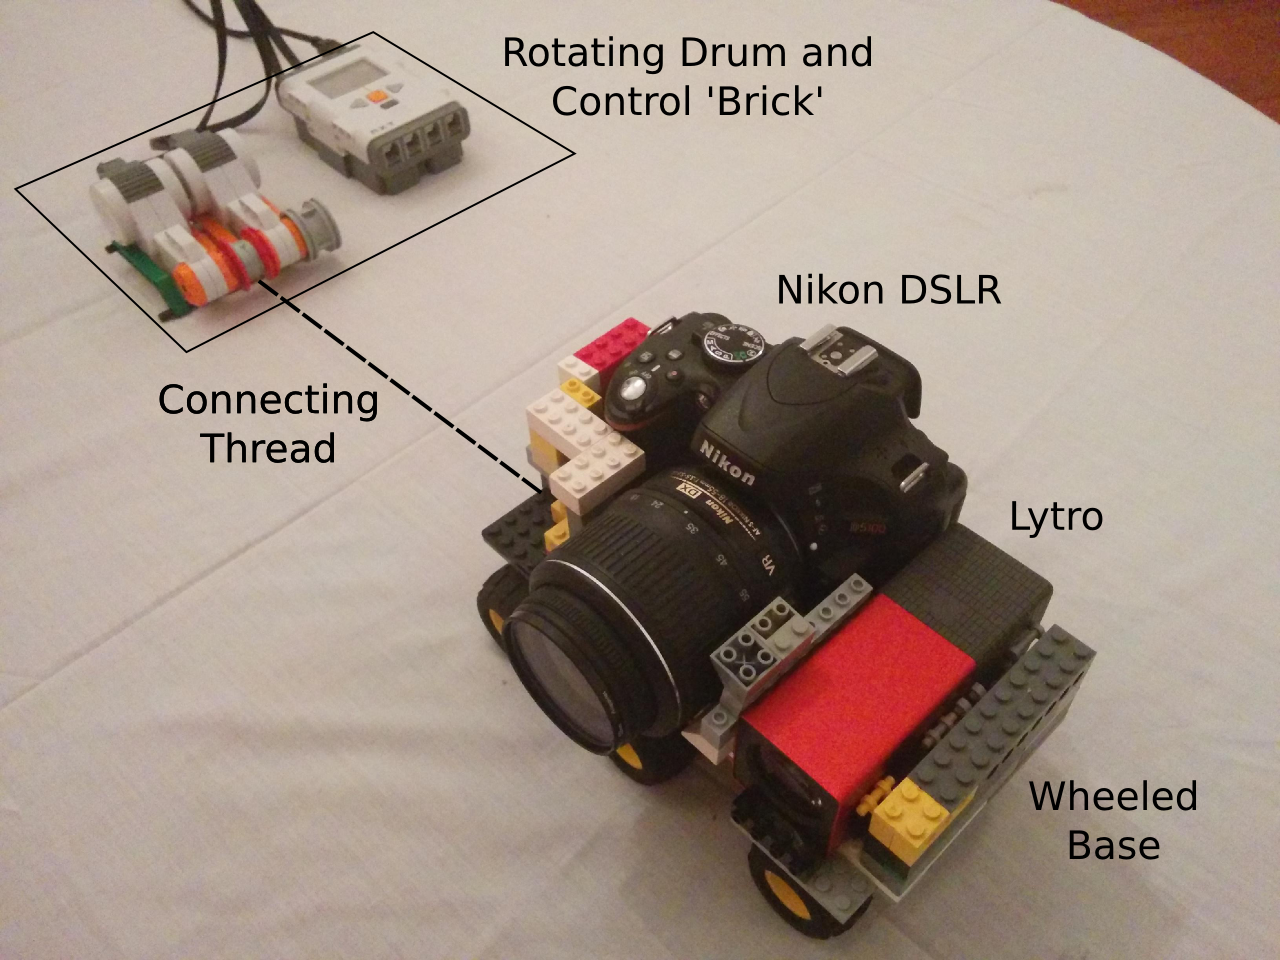
\includegraphics[width=\textwidth]{motion_platform}
\caption[Linear motion platform design]{Linear motion platform design}
\label{fig:motion_platform}
\end{figure}


\section{Scene Design}
\label{sec:scene_design}

The photographic scenes were set up in a room with no external facing windows to ensure the scene brightness could be controlled.
Three 60 watt incandescent static ceiling lights were used for ambient lighting in conjunction with a single 72 watt diffuse incandescent light source placed behind the linear motion platform carrying the cameras..
The 72 watt light source was placed facing front-on to the scene to reduce visible shadow size.
A plain white covering was placed on the working surface to reflect extra ambient light.

A large board was placed behind the scene to provide a constant background depth and scene elements were elevated using platforms where necessary.
The scenes used had a depth range (distance from the front of the Lytro camera to the background plane) of up to 40cm.
Figure \ref{fig:scene_description} shows the experimental scene configuration.

\begin{figure}[h]
\centering
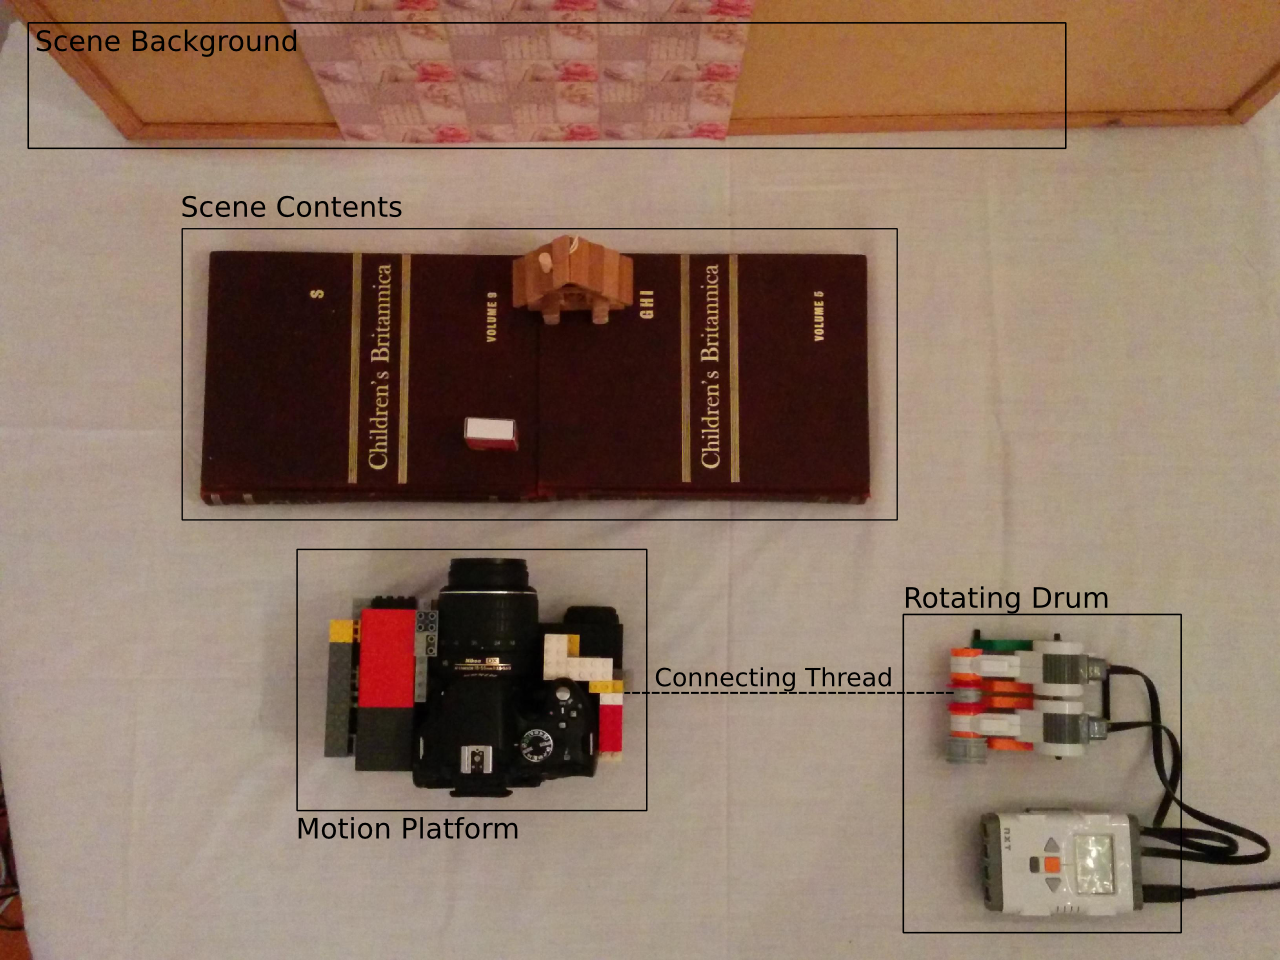
\includegraphics[width=\textwidth]{scene_contents}
\caption[Experimental scene layout]{Experimental scene layout, shown from above}
\label{fig:scene_description}
\end{figure}


\section{Image Capture}
\label{sec:image_capture}

A Lytro camera with firmware version 1.2.2 was used for the light field photography.
The Lytro camera was configured using the following settings.

\begin{table}[h]
\centering
\caption{Lytro Camera Settings}
\label{tab:lytro_settings}
\begin{tabular}{r | l}
Zoom & 1.0 \\
Creative Mode & Off \\
ND Filter & Off \\
ISO Sensitivity & Auto \\
Shutter Speed & As Required \\
Shutter Delay & 10s \\
\end{tabular}
\end{table}

The shutter delay was set to 10s to allow the motion platform to reach a stable velocity before the picture was taken.
Once the camera countdown was started, the motion platform was initiated from a Laptop running Matlab version R2009 and the RWHT Mindstorms Toolbox \cite{rwth2007toolbox}.

Images were transfered to an computer using the standard Lytro Desktop companion software (version 3.1.1 for OSX).
A 2011 model Apple Mac Book Air running OSX 10.9.3 was used for image processing.
Version 0.2 of the Light Field Toolbox \cite{dansereau2013toolbox} was used for light field manipulation and processing in Matlab.
The image decoding process used by the LF toolbox is described in \cite{dansereau2013decoding}.

Lytro \enquote*{.lfp} files were converted to raw image files and metadata files using the python-lfp-reader Python scripts (version 0.2) \cite{esfahbod2013python}, as per the Matlab LF Toolbox instructions \cite{dansereau2013toolbox}.

\section{Image Processing and Deconvolution}
\label{sec:image_processing_and_deconvolution}

The raw image files were read using the Matlab LF Toolbox, as described in \cite{dansereau2013toolbox}.
The Lytro depth maps were extracted from the Lytro desktop software image database using the python-lfp-reader Python scripts \cite{esfahbod2013python}.

Camera velocity was measured using the Lego Mindstorms motor encoders on the motion platform after initial calibration of the platform.

The exposure time and focal length were read from the Lytro image metadata, and a scaling factor for the Lytro focal length determined experimentally by comparing observed blur lengths with metric depths, using equation \ref{eq:blur_width_simple}.

To de-blur the light field, all possible sup-aperture slices were taken and individually deconvoled once at every scene depth.
This was done using the Richardson-Lucy method due to it's relatively quick processing time and characteristically good performance.
The Matlab \enquote*{deconvlucy} command was used for the Richardson-Lucy de-blurring implementation.
The deconvoled sub-aperture images were then combined, using image masks computed for each depth map depth.
The deblurred sub-aperture images were combined such that an optimal PSF was used for each pixel within the final image.
This Matlab code for this process is fully described in Appendix XXXX.


\section{Analysis}
\label{sec:analysis}

Two quantitative measures were used to compare de-blurred light fields.
A \enquote*{Q-Factor} was computed to measure the increase in image sharpness and the Root-Mean-Square Error (RMSE) was estimated to measure the degree of noise amplification introduced by the deconvolution.

Without a ground truth image, a simple and well defined measure of \enquote*{image sharpness} is not easy to formulate, as evidenced by the complexity of image sharpness standards \cite{imatest2014sharpness}.
The original intention was to use the DSLR camera for capturing ground truth images, however due to the short depth range within the scene, the DSLR camera was unable to focus on all objects within the scene.
As such, a Q-factor had to be derived without access to a ground truth image.
The Q-factor definition used met this requirement and served to demonstrate the quantifiable recovery of high-frequency image content after de-blurring.

The Q-Factor used here was computed by summing absolute pixel intensities after applying a vertical Prewitt edge detection filter.
These sums were then normalised relative to the original blurred image Q-factor.
This had the effect of measuring the increase in the intensity of high-frequency components in the image.
Thus, the Q-factor we used was

\begin{equation}
Q = \frac{\sum_{x=1}^{W} \sum_{y=1}^{H}
\left| (I \ast G)(x, y) \right|
\label{eq:q_factor}}{Q_b}
\end{equation}

\noindent
where $Q_b$ is the Q-Factor for the original image, $W$ and $H$ are the width and height of the image, $I$ is the de-blurred image, and $G$ is the Prewitt vertical edge detection kernel;

\begin{equation}
G = 
\begin{bmatrix}
1 & 0 & -1 \\
1 & 0 & -1 \\
1 & 0 & -1 \\
\end{bmatrix}
\label{eq:prewitt_filter}
\end{equation}

\noindent
(the vertical detection kernel was used due to the presence of horizontal motion blur in the tests performed here).
This Q-factor definition had the downside of also measuring noise content.
Thus, noisy images could potentially score higher than clean, sharp images.
To account for this, and provide a more balanced measure of de-blurring performance, the RMSE noise estimate was also used to compare de-blurred images.

The RMSE noise was estimated by converting the central sub-aperture image to grayscale, then manually cropping out a small (approximately 50x50 pixel) region known to be of constant color.
The RMSE was then computed using

\begin{equation}
R = \sqrt{ \sum_{x=1}^{W} \sum_{y=1}^{H} (I(x,y) - m)^2 }
\end{equation}

\noindent
where $W$ and $H$ are the width and height of the region respectively, $I$ is the region image and $m$ is the mean gray level within the region.
This metric gives an estimate of the additive noise content in the image prior to de-blurring, and an estimate of the noise (ringing and additive) in the image after de-blurring.

